\documentclass{article}


\usepackage{bytefield}
\usepackage{tikz}
\usetikzlibrary{positioning}


\setlength{\parindent}{0pt}
\setlength{\parskip}{1em}


\begin{document}

\title{Instruction Set Architecture}
\author{Jonathan Uhler}
\date{\today}
\maketitle

\textbf{Abstract}
This document describes a simple RISC instruction set architecture designed to learn more about
computer architecture.
\pagebreak


\section{Registers}
This section describes information about all the registers in the processor.

All registers in this architecture are 16 bits wide. Integral values are presumed to be signed with
two's complement encoding unless otherwise specified by certain unsigned-specific instructions.
Some registers, like status registers, have no concept of signedness.

\subsection{General Purpose Registers}
The following general purpose registers exist in the register file, with the recommended ABI
assignments.

\begin{tabular}{|cclc|}
  \hline
  Register & ABI Name & Use & Saver \\
  \hline
  r0 & zero & Hard-wired zero & N/A \\
  r1 & ra & Return address (absolute byte address) & Caller \\
  r2 & sp & Stack pointer (absolute byte address) & Callee \\
  r3 - r10 & a0 - a7 & Arguments and return values & Caller \\
  r11 - r18 & t0 - t7 & Temporary values & Caller \\
  r19 - r31 & s0 - s12 & Saved values & Callee \\
  \hline
\end{tabular}

\subsection{Control and Status Registers}
The following special registers also exist, but are not directly accessible by the same
instructions as general purpose registers. Certain instructions may include hardware to modify
these registers. The control flow itself may also modify these registers as time passes.

\begin{tabular}{|cp{10cm}|}
  \hline
  Register & Use \\
  \hline
  pc & Program counter (absolute byte address) \\
  reset & ONE when the processor is in reset, ZERO otherwise, set by the halt instruction \\
  \hline
\end{tabular}


\section{Memory}
Registers in this architecture are 16 bits wide, and addresses (stored in registers) are always
absolute. Thus, the maximum usable memeory is 64KB. Future extensions may add instructions
to manager memory page indexing, allowing a larger window of memory to be used (although at a
performance cost).

Note that only the red regions are required. The rest of the memory map for code, stack, and heap
can be changed.

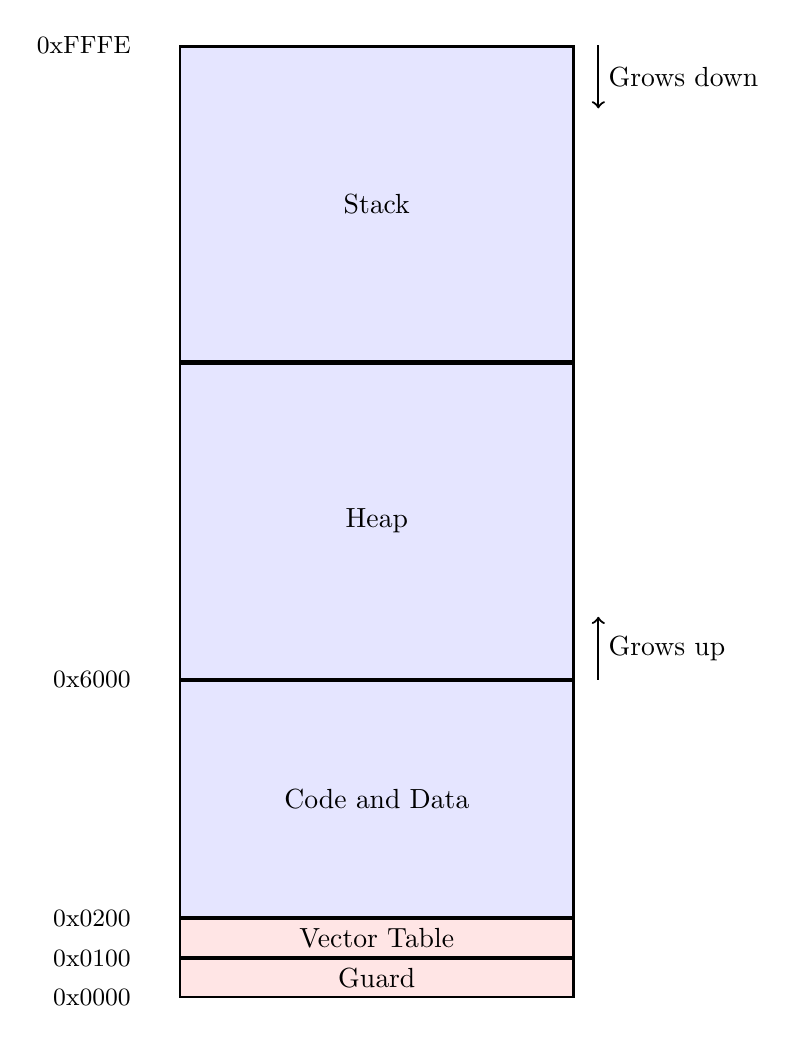
\begin{tikzpicture}[
  segment/.style={draw, thick, minimum width=5cm, align=center},
  label/.style={font=\small}
]

\node[segment, fill=blue!10, minimum height=4cm] (stack) {Stack};
\node[segment, fill=blue!10, minimum height=4cm, below=0pt of stack] (heap) {Heap};
\node[segment, fill=blue!10, minimum height=3cm, below=0pt of heap] (code) {Code and Data};
\node[segment, fill=red!10, below=0pt of code] (vector_table) {Vector Table};
\node[segment, fill=red!10, below=0pt of vector_table] (guard) {Guard};

\draw[->, thick] (stack.north east) ++(0.3,0) -- ++(0,-0.8) node[midway, right]{Grows down};
\draw[->, thick] (heap.south east) ++(0.3,0) -- ++(0,0.8) node[midway, right]{Grows up};

\node[label, left=3cm of stack.north] {0xFFFE};
\node[label, left=3cm of heap.south] {0x6000};
\node[label, left=3cm of code.south] {0x0200};
\node[label, left=3cm of vector_table.south] {0x0100};
\node[label, left=3cm of guard.south] {0x0000};
\end{tikzpicture}


\section{Core Instructions}
This section describes the minimum set of instructions that must be supported by a complete
implementation. Using these instructions, other convenience operations can be added as either
composite instructions or aliases (see the Pseudo Instructions section for more information).

\subsection{Instruction Formats}
This instruction set defines several different formats used to decode instructions based on the
list of operands that they take. These are listed in order below by the number of register operands
taken.

Instructions in this architecture are always fixed width, with no ``narrow'' formats as of yet. All
formats are encoded in little endian byte order, where bit 0 is the least-significant bit and bit 31
is the most-significant bit.

\subsubsection{I-Type}
Immediate-only instructions.

Used for instructions that take a single immediate operand and no register operands. These are
generally reserved for status and hardware control instructions (like halting the processor).

The Format field (bit 1:0) of I-type instructions is \verb|00|.

\begin{bytefield}[bitwidth=0.4cm]{32}
  \bitheader[endianness=big]{0-31}
  \\
  \bitbox{16}{Immediate}
  \bitbox{10}{-}
  \bitbox{4}{Funct}
  \bitbox{2}{00}
\end{bytefield}

\subsubsection{DSI-Type}
Destination, source, and immediate instructions.

Used for instructions that perform an operation on a destination register based on the value in
a source (operand) register and an immediate value. This is a common format for any binary operation
which takes an immediate.

The Format field (bit 1:0) of DSI-type instructions is \verb|10|.

\begin{bytefield}[bitwidth=0.4cm]{32}
  \bitheader[endianness=big]{0-31}
  \\
  \bitbox{16}{Immediate}
  \bitbox{5}{Source 1}
  \bitbox{5}{Dest}
  \bitbox{4}{Funct}
  \bitbox{2}{10}
\end{bytefield}

\subsubsection{DSS-Type}
Destination, source, and source instructions.

Used for instructions that perform an operation on a destination register based on the values in two
source registers. This is a common format for any binary operation that operates exclusively with
registers.

The Format field (bit 1:0) of DSS-type instructions is \verb|11|.

\begin{bytefield}[bitwidth=0.4cm]{32}
  \bitheader[endianness=big]{0-31}
  \\
  \bitbox{11}{-}
  \bitbox{5}{Source 2}
  \bitbox{5}{Source 1}
  \bitbox{5}{Dest}
  \bitbox{4}{Funct}
  \bitbox{2}{11}
\end{bytefield}

\subsection{Instruction List}
The minumum core instructions for a full implementation of this architecture, organized
alphabetically, are as follows.

This specification makes no recommendation on whether these instructions are implemented with
separate hardware units or as pseudo instructions (where possible). All of these instructions must
exist and perform the specified operation for a full implementation.

In the ``Meaning'' section of each instruction, the \verb|R| object refers to the register file,
which is indexed with the number of a register (0 through31). The \verb|M| object is main memory,
which is byte-addressable.

\subsubsection{ADD - Addition}
\begin{bytefield}[bitwidth=0.4cm]{32}
  \bitheader[endianness=big]{0-31}
  \\
  \bitbox{11}{-}
  \bitbox{5}{Source 2}
  \bitbox{5}{Source 1}
  \bitbox{5}{Dest}
  \bitbox{4}{0000}
  \bitbox{2}{11}
\end{bytefield}

Meaning: \verb|R[Dest] <- R[Source1] + R[Source2]|

Assembler format: \verb|add rd, rs1, rs2|

Add Source 1 and Source 2 and store the result in Dest.

\subsubsection{ADDI - Addition With Immediate}
\begin{bytefield}[bitwidth=0.4cm]{32}
  \bitheader[endianness=big]{0-31}
  \\
  \bitbox{16}{Immediate}
  \bitbox{5}{Source 1}
  \bitbox{5}{Dest}
  \bitbox{4}{0000}
  \bitbox{2}{10}
\end{bytefield}

Meaning: \verb|R[Dest] <- R[Source1] + Immediate|

Assembler format: \verb|addi rd, rs1, imm|

Add Source 1 and Immediate and store the result in Dest.

\subsubsection{AND - Bitwise And}
\begin{bytefield}[bitwidth=0.4cm]{32}
  \bitheader[endianness=big]{0-31}
  \\
  \bitbox{11}{-}
  \bitbox{5}{Source 2}
  \bitbox{5}{Source 1}
  \bitbox{5}{Dest}
  \bitbox{4}{0010}
  \bitbox{2}{11}
\end{bytefield}

Meaning: \verb|R[Dest] <- R[Source1] & R[Source2]|

Assembler format: \verb|and rd, rs1, rs2|

Compute the bitwise AND of Source 1 and Source 2 and store the result in Dest.

\subsubsection{ANDI - Bitwise And With Immediate}
\begin{bytefield}[bitwidth=0.4cm]{32}
  \bitheader[endianness=big]{0-31}
  \\
  \bitbox{16}{Immediate}
  \bitbox{5}{Source 1}
  \bitbox{5}{Dest}
  \bitbox{4}{0010}
  \bitbox{2}{10}
\end{bytefield}

Meaning: \verb|R[Dest] <- R[Source1] & Immediate|

Assembler format: \verb|andi rd, rs1, imm|

Compute the bitwise AND of Source 1 and Immediate and store the result in Dest.

\subsubsection{EQ - Equals}
\begin{bytefield}[bitwidth=0.4cm]{32}
  \bitheader[endianness=big]{0-31}
  \\
  \bitbox{11}{-}
  \bitbox{5}{Source 2}
  \bitbox{5}{Source 1}
  \bitbox{5}{Dest}
  \bitbox{4}{1000}
  \bitbox{2}{11}
\end{bytefield}

Meaning: \verb|R[Dest] <- R[Source1] == R[Source2]|

Assembler format: \verb|eq rd, rs1, rs2|

If Source 1 and Source 2 are equal, store ONE in Dest, else store ZERO in Dest.

\subsubsection{GT - Greater Than}
\begin{bytefield}[bitwidth=0.4cm]{32}
  \bitheader[endianness=big]{0-31}
  \\
  \bitbox{11}{-}
  \bitbox{5}{Source 2}
  \bitbox{5}{Source 1}
  \bitbox{5}{Dest}
  \bitbox{4}{1001}
  \bitbox{2}{11}
\end{bytefield}

Meaning: \verb|R[Dest] <- R[Source1] > R[Source2]|

Assembler format: \verb|gt rd, rs1, rs2|

If Source 1 is greater than Source 2, store ONE in Dest, else store ZERO in Dest.

\subsubsection{HALT - Halt Processor}
\begin{bytefield}[bitwidth=0.4cm]{32}
  \bitheader[endianness=big]{0-31}
  \\
  \bitbox{16}{Immediate}
  \bitbox{10}{-}
  \bitbox{4}{0000}
  \bitbox{2}{00}
\end{bytefield}

Meaning: \verb|exit(Immediate)|

Assembler format: \verb|halt imm|

Halt processor execution with the exit code in Immediate until reset is next released.

\subsubsection{JLO - Jump and Link on One}
\begin{bytefield}[bitwidth=0.4cm]{32}
  \bitheader[endianness=big]{0-31}
  \\
  \bitbox{16}{Immediate}
  \bitbox{5}{Source 1}
  \bitbox{5}{Dest}
  \bitbox{4}{1111}
  \bitbox{2}{10}
\end{bytefield}

Meaning: \verb|if (R[Source1] == 1) { R[Dest] <- PC + 4; PC <- Immediate }|

Assembler format: \verb|jlo rd, rs1, imm|

If Source 1 is ONE, store the address of the next instruction in Dest and jump to the absolute
address in Immediate.

\subsubsection{JLRO - Jump and Link Register on One}
\begin{bytefield}[bitwidth=0.4cm]{32}
  \bitheader[endianness=big]{0-31}
  \\
  \bitbox{11}{-}
  \bitbox{5}{Source 2}
  \bitbox{5}{Source 1}
  \bitbox{5}{Dest}
  \bitbox{4}{1111}
  \bitbox{2}{11}
\end{bytefield}

Meaning: \verb|if (R[Source1] == 1) { R[Dest] <- PC + 4; PC <- R[Source2] }|

Assembler format: \verb|jlro rd, rs1, rs2|

If Source 1 is ONE, store the address of the next instruction in Dest and jump to the absolute
address in Source 2.

\subsubsection{JLRZ - Jump and Link Register on Zero}
\begin{bytefield}[bitwidth=0.4cm]{32}
  \bitheader[endianness=big]{0-31}
  \\
  \bitbox{11}{-}
  \bitbox{5}{Source 2}
  \bitbox{5}{Source 1}
  \bitbox{5}{Dest}
  \bitbox{4}{1110}
  \bitbox{2}{11}
\end{bytefield}

Meaning: \verb|if (R[Source1] == 0) { R[Dest] <- PC + 4; PC <- R[Source2] }|

Assembler format: \verb|jlrz rd, rs1, rs2|

If Source 1 is ZERO, store the address of the next instruction in Dest and jump to the absolute
address in Source 2.

\subsubsection{JLZ - Jump and Link on Zero}
\begin{bytefield}[bitwidth=0.4cm]{32}
  \bitheader[endianness=big]{0-31}
  \\
  \bitbox{16}{Immediate}
  \bitbox{5}{Source 1}
  \bitbox{5}{Dest}
  \bitbox{4}{1110}
  \bitbox{2}{10}
\end{bytefield}

Meaning: \verb|if (R[Source1] == 0) { R[Dest] <- PC + 4; PC <- Immediate }|

Assembler format: \verb|jlz rd, rs1, imm|

If Source 1 is ZERO, store the address of the next instruction in Dest and jump to the absolute
address in Immediate.

\subsubsection{LD - Load}
\begin{bytefield}[bitwidth=0.4cm]{32}
  \bitheader[endianness=big]{0-31}
  \\
  \bitbox{16}{Immediate}
  \bitbox{5}{Source 1}
  \bitbox{5}{Dest}
  \bitbox{4}{1100}
  \bitbox{2}{10}
\end{bytefield}

Meaning: \verb|R[Dest] <- M[R[Source1] + Immediate]|

Assembler format: \verb|ld rd, rs1, imm|

Load 16 bits from the address formed by adding Source 1 and Immediate and store the value in Dest.

\subsubsection{LT - Less Than}
\begin{bytefield}[bitwidth=0.4cm]{32}
  \bitheader[endianness=big]{0-31}
  \\
  \bitbox{11}{-}
  \bitbox{5}{Source 2}
  \bitbox{5}{Source 1}
  \bitbox{5}{Dest}
  \bitbox{4}{1010}
  \bitbox{2}{11}
\end{bytefield}

Meaning: \verb|R[Dest] <- R[Source1] < R[Source2]|

Assembler format: \verb|lt rd, rs1, rs2|

If Source 1 is less than Source 2, store ONE in Dest, else store ZERO in Dest.

\subsubsection{NE - Not Equal}
\begin{bytefield}[bitwidth=0.4cm]{32}
  \bitheader[endianness=big]{0-31}
  \\
  \bitbox{11}{-}
  \bitbox{5}{Source 2}
  \bitbox{5}{Source 1}
  \bitbox{5}{Dest}
  \bitbox{4}{1011}
  \bitbox{2}{11}
\end{bytefield}

Meaning: \verb|R[Dest] <- R[Source1] != R[Source2]|

Assembler format: \verb|ne rd, rs1, rs2|

If Source 1 is not equal to Source 2, store ONE in Dest, else store ZERO in Dest.

\subsubsection{OR - Bitwise Or}
\begin{bytefield}[bitwidth=0.4cm]{32}
  \bitheader[endianness=big]{0-31}
  \\
  \bitbox{11}{-}
  \bitbox{5}{Source 2}
  \bitbox{5}{Source 1}
  \bitbox{5}{Dest}
  \bitbox{4}{0011}
  \bitbox{2}{11}
\end{bytefield}

Meaning: \verb/R[Dest] <- R[Source1] | R[Source2]/

Assembler format: \verb|or rd, rs1, rs2|

Compute the bitwise OR of Source 1 and Source 2 and store the result in Dest.

\subsubsection{ORI - Bitwise Or With Immediate}
\begin{bytefield}[bitwidth=0.4cm]{32}
  \bitheader[endianness=big]{0-31}
  \\
  \bitbox{16}{Immediate}
  \bitbox{5}{Source 1}
  \bitbox{5}{Dest}
  \bitbox{4}{0011}
  \bitbox{2}{10}
\end{bytefield}

Meaning: \verb/R[Dest] <- R[Source1] | Immediate/

Assembler format: \verb|ori rd, rs1, imm|

Compute the bitwise OR of Source 1 and Immediate and store the result in Dest.

\subsubsection{SLL - Logical Shift Left}
\begin{bytefield}[bitwidth=0.4cm]{32}
  \bitheader[endianness=big]{0-31}
  \\
  \bitbox{11}{-}
  \bitbox{5}{Source 2}
  \bitbox{5}{Source 1}
  \bitbox{5}{Dest}
  \bitbox{4}{0101}
  \bitbox{2}{11}
\end{bytefield}

Meaning: \verb|R[Dest] <- R[Source1] << R[Source2]|

Assembler format: \verb|sll rd, rs1, rs2|

Shift Source 1 left by Source 2 bits and store the result in Dest.

\subsubsection{SLLI - Logical Shift Left by Immediate}
\begin{bytefield}[bitwidth=0.4cm]{32}
  \bitheader[endianness=big]{0-31}
  \\
  \bitbox{16}{Immediate}
  \bitbox{5}{Source 1}
  \bitbox{5}{Dest}
  \bitbox{4}{0101}
  \bitbox{2}{10}
\end{bytefield}

Meaning: \verb|R[Dest] <- R[Source1] << Immediate|

Assembler format: \verb|slli rd, rs1, imm|

Shift Source 1 left by Immediate bits and store the result in Dest.

\subsubsection{SRA - Arithmetic Shift Right}
\begin{bytefield}[bitwidth=0.4cm]{32}
  \bitheader[endianness=big]{0-31}
  \\
  \bitbox{11}{-}
  \bitbox{5}{Source 2}
  \bitbox{5}{Source 1}
  \bitbox{5}{Dest}
  \bitbox{4}{0111}
  \bitbox{2}{11}
\end{bytefield}

Meaning: \verb|R[Dest] <- (int) R[Source1] >> R[Source2]|

Assembler format: \verb|sra rd, rs1, rs2|

Shift Source 1 right with SIGN extension by Source 2 bits and store the result in Dest.

\subsubsection{SRAI - Arithmetic Shift Right by Immediate}
\begin{bytefield}[bitwidth=0.4cm]{32}
  \bitheader[endianness=big]{0-31}
  \\
  \bitbox{16}{Immediate}
  \bitbox{5}{Source 1}
  \bitbox{5}{Dest}
  \bitbox{4}{0111}
  \bitbox{2}{10}
\end{bytefield}

Meaning: \verb|R[Dest] <- (int) R[Source1] >> Immediate|

Assembler format: \verb|srai rd, rs1, imm|

Shift Source 1 right with SIGN extension by Immediate bits and store the result in Dest.

\subsubsection{SRL - Logical Shift Right}
\begin{bytefield}[bitwidth=0.4cm]{32}
  \bitheader[endianness=big]{0-31}
  \\
  \bitbox{11}{-}
  \bitbox{5}{Source 2}
  \bitbox{5}{Source 1}
  \bitbox{5}{Dest}
  \bitbox{4}{0110}
  \bitbox{2}{11}
\end{bytefield}

Meaning: \verb|R[Dest] <- (uint) R[Source1] >> R[Source2]|

Assembler format: \verb|srl rd, rs1, rs2|

Shift Source 1 right with ZERO extension by Source 2 bits and store the result in Dest.

\subsubsection{SRLI - Logical Shift Right by Immediate}
\begin{bytefield}[bitwidth=0.4cm]{32}
  \bitheader[endianness=big]{0-31}
  \\
  \bitbox{16}{Immediate}
  \bitbox{5}{Source 1}
  \bitbox{5}{Dest}
  \bitbox{4}{0110}
  \bitbox{2}{10}
\end{bytefield}

Meaning: \verb|R[Dest] <- (uint) R[Source1] >> Immediate|

Assembler format: \verb|srli rd, rs1, imm|

Shift Source 1 right with ZERO extension by Immediate bits and store the result in Dest.

\subsubsection{ST - Store}
\begin{bytefield}[bitwidth=0.4cm]{32}
  \bitheader[endianness=big]{0-31}
  \\
  \bitbox{16}{Immediate}
  \bitbox{5}{Source 1}
  \bitbox{5}{Dest}
  \bitbox{4}{1101}
  \bitbox{2}{10}
\end{bytefield}

Meaning: \verb|M[R[Source1] + Immediate] <- R[Dest]|

Assembler format: \verb|st rd, rs1, imm|

Store Dest into the address formed by adding Source 1 and Immediate.

\subsubsection{SUB - Subtraction}
\begin{bytefield}[bitwidth=0.4cm]{32}
  \bitheader[endianness=big]{0-31}
  \\
  \bitbox{11}{-}
  \bitbox{5}{Source 2}
  \bitbox{5}{Source 1}
  \bitbox{5}{Dest}
  \bitbox{4}{0001}
  \bitbox{2}{11}
\end{bytefield}

Meaning: \verb|R[Dest] <- R[Source1] - R[Source2]|

Assembler format: \verb|sub rd, rs1, rs2|

Subtract Source 2 from Source 1 and store the result in Dest.

\subsubsection{SUBI - Subtraction With Immediate}
\begin{bytefield}[bitwidth=0.4cm]{32}
  \bitheader[endianness=big]{0-31}
  \\
  \bitbox{16}{Immediate}
  \bitbox{5}{Source 1}
  \bitbox{5}{Dest}
  \bitbox{4}{0001}
  \bitbox{2}{10}
\end{bytefield}

Meaning: \verb|R[Dest] <- R[Source1] - Immediate|

Assembler format: \verb|subi rd, rs1, imm|

Subtract Immediate from Source 1 and store the result in Dest.

\subsubsection{XOR - Bitwise Exclusive Or}
\begin{bytefield}[bitwidth=0.4cm]{32}
  \bitheader[endianness=big]{0-31}
  \\
  \bitbox{11}{-}
  \bitbox{5}{Source 2}
  \bitbox{5}{Source 1}
  \bitbox{5}{Dest}
  \bitbox{4}{0100}
  \bitbox{2}{11}
\end{bytefield}

Meaning: \verb/R[Dest] <- R[Source1] ^ R[Source2]/

Assembler format: \verb|xor rd, rs1, rs2|

Compute the bitwise XOR of Source 1 and Source 2 and store the result in Dest.

\subsubsection{XORI - Bitwise Exclusive Or With Immediate}
\begin{bytefield}[bitwidth=0.4cm]{32}
  \bitheader[endianness=big]{0-31}
  \\
  \bitbox{16}{Immediate}
  \bitbox{5}{Source 1}
  \bitbox{5}{Dest}
  \bitbox{4}{0100}
  \bitbox{2}{10}
\end{bytefield}

Meaning: \verb/R[Dest] <- R[Source1] ^ Immediate/

Assembler format: \verb|xori rd, rs1, imm|

Compute the bitwise XOR of Source 1 and Immediate and store the result in Dest.

\subsection{Opcode Table}
An alternative way of viewing the core instructions is by looking at their Format and Funct bits,
which together form a single operation code (opcode).

Each row corresponds to a Format code (bits 1:0 of an instruction) and each column corresponds to
a Funct code (bits 5:2 of an instruction). The Format code \verb|01| is currently reserved and
contains no valid instructions.

The top six bits of an instruction (bits 5:0) can be read by indexing the column first, then the
row.

\noindent\makebox[\textwidth][c]{
\begin{tabular}{c|c|c|c|c|c|c|c|c|c|c|c|c|c|c|c|c|}
     & 0000 & 0001 & 0010 & 0011 & 0100 & 0101 & 0110 & 0111 & 1000 & 1001 & 1010 & 1011 & 1100 & 1101 & 1110 & 1111 \\
  \hline
  00 & halt &      &      &      &      &      &      &      &      &      &      &      &      &      &      &      \\
  01 &      &      &      &      &      &      &      &      &      &      &      &      &      &      &      &      \\
  10 & addi & subi & andi & ori  & xori & slli & srli & srai &      &      &      &      & ld   & st   & jlz  & jlo  \\
  11 & add  & sub  & and  & or   & xor  & sll  & srl  & sra  & eq   & gt   & lt   & ne   &      &      & jlrz & jlro
\end{tabular}
}


\section{Pseudo Instructions}
Additional convenience instructions can be created from the minimum required core instructions.
These are not mandatory for a full implementation, but can be nice extensions for assemblers and
may make code more readable.

Multiple logically equivalent implementations may exist for these pseudo instructions using the
core instruction set. The listed implementation is the canonical implementation.

\subsection{Instruction List}

\subsubsection{J - Unconditional Jump}
Meaning: \verb|PC <- Immediate|

Assembler format: \verb|j imm|

Implementation: \verb|jlz r0, r0, imm|

Unconditionally jump to absolute address in Immediate.

\subsubsection{JL - Unconditional Jump and Link}
Meaning: \verb|R[Dest] <- PC + 4; PC <- Immediate|

Assembler format: \verb|jl rd, imm|

Implementation: \verb|jlz rd, r0, imm|

Unconditionally store the address of the next instruction in Dest and jump to the absolute
address in Immediate.

\subsubsection{JLR - Unconditional Jump and Link Register}
Meaning: \verb|R[Dest] <- PC + 4; PC <- R[Source1]|

Assembler format: \verb|jlr rd, rs1|

Implementation: \verb|jlrz rd, r0, rs1|

Unconditionally store the address of the next instruction in Dest and jump to the absolute
address in Source 1.

\subsubsection{JO - Jump on One}
Meaning: \verb|if (R[Source1] == 1) { PC <- Immediate }|

Assembler format: \verb|jo rs1, imm|

Implementation: \verb|jlo r0, rs1, imm|

If Source 1 is ONE, jump to the absolute address in Immediate.

\subsubsection{JZ - Jump on Zero}
Meaning: \verb|if (R[Source1] == 0) { PC <- Immediate }|

Assembler format: \verb|jz rs1, imm|

Implementation: \verb|jlz r0, rs1, imm|

If Source 1 is ZERO, jump to the absolute address in Immediate.

\subsubsection{CALL - Call Subroutine}
Meaning: \verb|RA <- PC + 4; PC <- Immediate|

Assembler format: \verb|call imm|

Implementation: \verb|jlz ra, r0, imm|

Jump to Immediate and store the address of the next instruction in the return address register.

\subsubsection{LI - Load Immediate}
Meaning: \verb|R[Dest] <- Immediate|

Assembler format: \verb|li rd, imm|

Implementation: \verb|ori rd, r0, imm|

Store the value in Immediate in Dest.

\subsubsection{MV - Move}
Meaning: \verb|R[Dest] <- R[Source1]|

Assembler format: \verb|mv rd, rs1|

Implementation: \verb|or rd, rs1, r0|

Store the value in Source 1 in Dest.

\subsubsection{NOP - No Operation}
Meaning: \verb|;|

Assembler format: \verb|nop|

Implementation: \verb|or r0, r0, r0|

Do nothing.

\subsubsection{RET - Return From Subroutine}
Meaning: \verb|PC <- RA|

Assembler format: \verb|ret|

Implementation: \verb|jlrz r0, r0, ra|

Jump to the value in the return address register.

\end{document}
